\bookchapter{第四十九章：開発環境を整える——Android Studioと最初のプロジェクト}

\chapterintro{仕事を仕上げるには、まず道具をととのえること。この章では「キッチン」を組み立てます。Android Studioを入れて、エミュレータを動かし、人生初のAndroidプロジェクトを作り、プロジェクト構造をほどいて覗いてみます。環境が整えば、自分の書いたコードが「押せるボタン」に変わる瞬間に、初めて出会えます——この瞬間を一生覚えているという人は少なくありません。}

\booksection{Android Studioをインストールする}

Android StudioはGoogle公式の統合開発環境（IDE）です。無料で、機能はフルセット。コードを書く、UIプレビューを見る、デバッグする、パッケージ化する——そのすべてがここに揃っています。インストールは4ステップです。

\begin{enumerate}
  \item 公式サイトdeveloper.android.com/studioを開き、最新の安定版をダウンロードします（2026年8月時点ではNarwhal以降のバージョン。Windows/Mac/Linux版があります）。
  \item インストーラを起動して、ひたすら「次へ」——セットアップウィザードがAndroid SDKとエミュレータのコンポーネントを自動で入れてくれます。
  \item 初回起動時に、案内に従ってSDKコンポーネントをダウンロードします（デフォルトのままでOK。数分と数GBの空き容量がいるかもしれません）。
  \item 終わるとウェルカム画面が現れます——おめでとうございます、「キッチン」の完成です。
\end{enumerate}

\begin{tcbwarn}{注意：ハードウェア要件を頭に入れておく}
Android Studioは「メモリを食べる」タイプです。メモリは16GBからがおすすめ（8GBでも動きますが、エミュレータを起動すると重くなりがち）。ディスクは20GB以上確保し、CPUが仮想化対応（BIOSでVT-x/AMD-Vを有効化）か確認しましょう。パソコンがどうしても古い場合は、エミュレータの代わりに「実機デバッグ」を使えば（この章の第4節で解説します）、むしろサクサク動きます。

\end{tcbwarn}

\booksection{最初のプロジェクトを作る}

ウェルカム画面でNew Projectをクリックし、Empty Activityテンプレート（いちばんすっきりした初心者向けテンプレート）を選んで、3つの項目を入力します。

\begin{center}
\begin{tabularx}{\linewidth}{|X|X|X|}
\hline
\textbf{設定項目} & \textbf{入力する内容} & \textbf{説明} \tabularnewline
\hline
Name & My First App & アプリ名。スマホのホーム画面に表示される \tabularnewline
Package name & com.example.myfirstapp & 世界で一意の識別子。慣習は「ドメインの逆書き」。まずはデフォルトのままで \tabularnewline
Minimum SDK & API 26（Android 8.0） & 最低サポートバージョン。95\%以上のデバイスをカバー \tabularnewline
\hline
\end{tabularx}
\end{center}

\begin{center}\small\color{gray}プロジェクト作成で入力する3つの項目\end{center}

Finishを押すと、Android StudioがGradleで依存関係を自動ダウンロードし、プロジェクトをビルドします（初回は数分待ちますが、2回目からはぐっと速くなります）。ビルドが終われば、動くアプリの完成です——まだ「Hello Android!」と1行表示するだけですが。

\begin{tcbinfo}{ワンポイント：パッケージ名のツボ}
パッケージ名（package name）はアプリの「身分証番号」のようなもので、世界中で重複が許されず、一度公開したら変更できません。個人の練習ならcom.example.xxxで十分。正式な製品では、自分のドメインの逆書き（com.あなたの名前.アプリ名 など）に変えます。com.exampleのままで公開すると——ストアに拒まれます。

\end{tcbinfo}

\booksection{動かしてみる：エミュレータと実機}

コードが書けたら、それを動かす「スマホ」が要ります。選択肢は2つ。

\booksubsection{エミュレータ（Emulator）}

エミュレータは、パソコンの中にAndroidスマホを1台仮想で作る仕組みです。Android StudioでDevice Manager Create Deviceと開き、端末を1台選び（Pixelシリーズがおすすめ） システムイメージを1つ選ぶ（Google APIs付きのもの） ダウンロード 起動します。そしてツールバーの緑の三角Runを押せば、数秒後に「スマホ」の画面にあなたのアプリが現れます。

\booksubsection{実機デバッグ（こちらがおすすめ）}

実機は、常にいちばんリアルなテスト環境です。スワイプの感触も、本物のネットワークも、本物のセンサーも、エミュレータでは真似できません。Androidの実機デバッグは簡単です。

\begin{enumerate}
  \item スマホで［設定］［端末情報］を開き、「ビルド番号」を7回連続タップして「開発者向けオプション」を有効にします。
  \item ［開発者向けオプション］でUSBデバッグをオンにします。
  \item USBケーブルでパソコンにつなぎ、スマホのポップアップで「USBデバッグを許可」を選びます。
  \item Android Studioに戻ると、ツールバーのデバイスのドロップダウンにあなたのスマホが現れるので、Runを押します。
\end{enumerate}

\textbf{落とし穴注意：USBデバッグはつけっぱなしにしない}\par

USBデバッグは、パソコンに「裏口」を開けておくようなものです。外で充電するときや、信用できないパソコンにつなぐときは、必ずUSBデバッグをオフにして、他人にデータを読まれないようにしましょう。普段の開発でも、使い終わったらオフにする。それを習慣にしてしまいましょう。

\booksection{プロジェクト構造の解体：各ファイルの役割}

プロジェクトを初めて開くと、左のファイルツリーに目が回るかもしれません。慌てないでください。日常の開発では、時間の90\%を次のいくつかのファイルだけで過ごすことになります。

\begin{center}
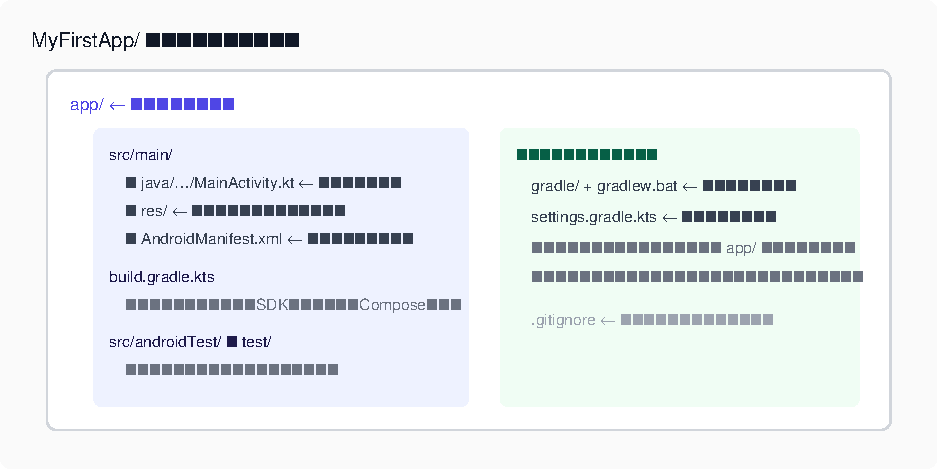
\includegraphics[width=0.92\linewidth]{figures/fig-di-si-shi-jiu-zhang-1}
\\[2pt]\small 図2：初心者が必ず知るプロジェクト構造（合言葉：触るのはapp/フォルダだけ）
\end{center}

\begin{itemize}
  \item MainActivity.kt：アプリの「玄関」です。ユーザーがアイコンをタップすると、最初に目覚めるのがこれ。今のテンプレートでは「Hello Android!」を表示する役割を担っています。
  \item AndroidManifest.xml：アプリの「住民票」です。このアプリの名前、アイコン、持っている画面、使う権限（カメラ、位置情報など）をここで宣言します。
  \item res/フォルダ：リソース倉庫。画像、アイコン、文字列、色を置きます。文字をコードに直書きせずリソースファイルに置くのは、Android開発の良い習慣です（言語やテーマの切り替えが楽になります）。
  \item build.gradle.kts：ビルドのレシピです。最低サポートバージョンや、依存するライブラリ（Composeなど）を宣言します。
\end{itemize}

\booksection{さっそく試す：「Hello」を自分の名前に変える}

MainActivity.ktを開くと、Composeテンプレートが生成したコードが見えます。Text(“Hello Android!”)という行を探し、引用符の中を自分の名前に変えてみましょう。たとえばText(“こんにちは、たろう！これは私の初めてのアプリです”)として、Ctrl+R（MacならCmd+R）で再実行します。数秒後、エミュレータにあなたの名前が表示されます。

\begin{lstlisting}[language=Kotlin]
setContent {
    MyFirstAppTheme {
        Surface(modifier = Modifier.fillMaxSize()) {
            // v ここを自分の好きな言葉に変えてみて
            Text("こんにちは、たろう！これは私の初めてのアプリです")
        }
    }
}
\end{lstlisting}

おめでとうございます。あなたは「コードを変える コンパイル インストール 実行」という1周のサイクルを完了しました。このサイクルこそ、これから毎日の開発の日常です。勢いに乗って、もう少し改造してみましょう。文字を大きくする、色を変える——次の章では、こうした「魔法」の正体を学びます。

\booksection{よくあるエラーの応急処置：初心者の最初2週間の「救急室」}

環境構築と初回ビルドの段階では、次の3種類のエラーにぶつかる可能性が高いでしょう。慌てないでください。どれにも効く薬があります。

\begin{center}
\begin{tabularx}{\linewidth}{|X|X|X|}
\hline
\textbf{エラーの症状} & \textbf{よくある原因} & \textbf{効く薬} \tabularnewline
\hline
Gradle sync failed／依存関係のダウンロードが遅い & リポジトリへのネットワーク接続が不安定 & Gradleに国内のミラーリポジトリ（Alibaba Cloud/Tencent Cloudのmavenミラー）を設定する。「Gradle ミラーリポジトリ 設定」などで検索し、手順どおりに直す \tabularnewline
SDKコンポーネントが足りない & インストール時にSDKのダウンロードをスキップした & Settings SDK Managerで、足りないプラットフォームとツールを追加インストール \tabularnewline
エミュレータが起動しない／真っ黒な画面 & 仮想化が無効、イメージの破損 & BIOSでVT-x/AMD-Vを有効化。エミュレータを削除して作り直す。または実機デバッグに切り替える \tabularnewline
\hline
\end{tabularx}
\end{center}

\begin{center}\small\color{gray}初心者向け環境エラー応急処置表\end{center}

\begin{tcbinfo}{ワンポイント：エラー検索の方法論}
エラーメッセージの1行目が、いちばん価値のある手がかりです。それをそのまま検索エンジンにコピーし、「android studio」のキーワードを添えましょう。「環境が入らないのですが」といった漠然とした言葉ではなく、「Gradle sync failed: Could not resolve com.android.tools.build」のような具体的なエラー文を検索します。正確な問いにだけ、正確な答えが返ってくるのです。

\end{tcbinfo}

\begin{tcbpractice}{やってみよう：「開発の儀式」リストを完成させる}
(1)Android Studioを入れてエミュレータを動かす。(2)自分のアプリを実機で1回動かし、スクリーンショットを残す。(3)Helloの文字を自分の名前に変える。(4)プロジェクトを圧縮して保存する。この4つが終わったら、友達にこう言えます。「私もAndroid開発者になったよ（証拠写真つきで）」。

\end{tcbpractice}

\begin{tcbsummary}{この章のまとめ}
\begin{itemize}
  \item Android Studio＝公式の無料IDE。メモリ16GB＋ディスク20GB＋仮想化の有効化がおすすめ
  \item 新規プロジェクトの3要素：名前、パッケージ名（世界で一意。com.exampleのまま公開しない）、最低SDK（API 26から）
  \item 実行方法は2つ：エミュレータ（パソコン内の仮想スマホ）と実機（USBデバッグをオン。使い終わったらオフに）
  \item プロジェクトの合言葉：触るのはapp/フォルダだけ——MainActivity.ktは玄関、Manifestは住民票、res/はリソース倉庫
  \item 開発の日常＝コードを変える Run 結果を見る、のくり返し
\end{itemize}

\end{tcbsummary}
